
% Inbuilt themes in beamer
\documentclass{beamer}
\usepackage{polski, xcolor, bookmark}

\newcommand{\comment}[1]{\textcolor{violet}{#1}}

% Theme choice:
\usetheme{default}

% Title page details: 
\title{O szukaniu dziury w całym}
\subtitle{Czyli analiza danych za pomocą topologii}
\author{Bartosz Furmanek}
\date{}


\begin{document}

% Title page frame
\begin{frame}
    \titlepage 
\end{frame}

% Outline frame
\begin{frame}{Program na dzisiaj}
    \tableofcontents
    Uwaga: \comment{fioletowe komentarze} służą do tego, żebym nie zapomniał niczego.
    Proszę zwracać mi uwagę, gdybym je zignorował!!!
    Wszystkie materiały są dostępne na GitHubie:
    \href{https://github.com/BartTheBartender/o-szukaniu-dziury-w-calym}{https://github.com/BartTheBartender/o-szukaniu-dziury-w-calym}.
\end{frame}

\section{Dlaczego?}
\begin{frame}{Datasaurus Dozen}
  \begin{center}
    \begin{tabular}{cccc}
      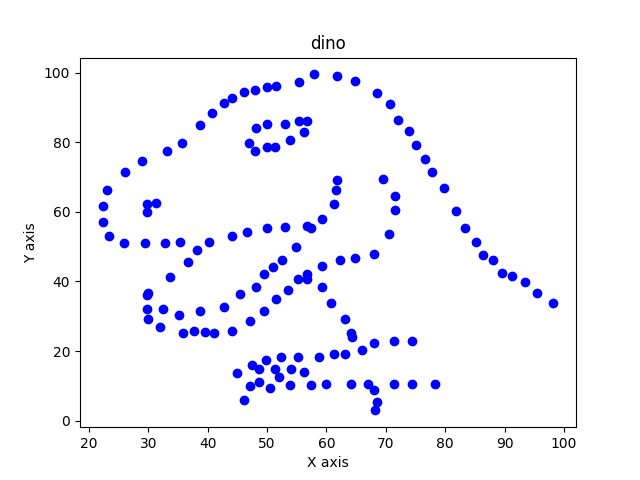
\includegraphics[width=0.20\textwidth]{images/datasaurus-0.png} &
      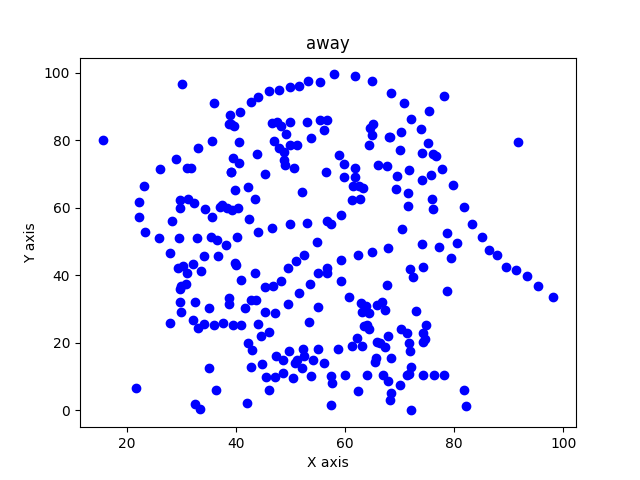
\includegraphics[width=0.20\textwidth]{images/datasaurus-1.png} &
      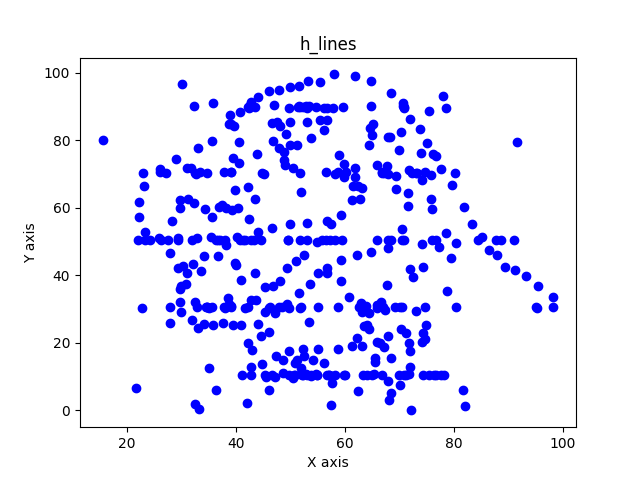
\includegraphics[width=0.20\textwidth]{images/datasaurus-2.png} &
      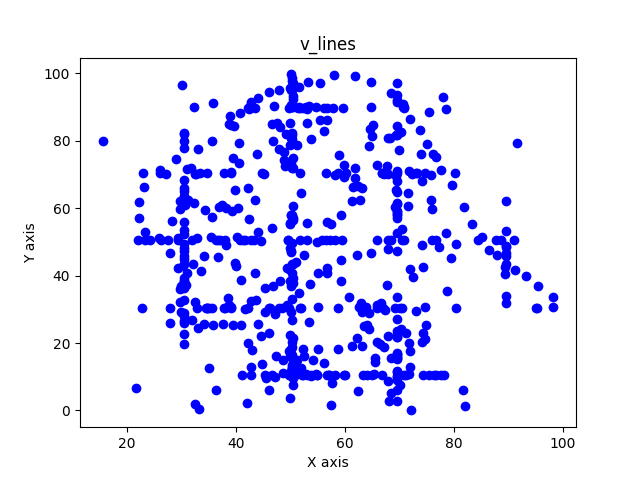
\includegraphics[width=0.20\textwidth]{images/datasaurus-3.png} \\
      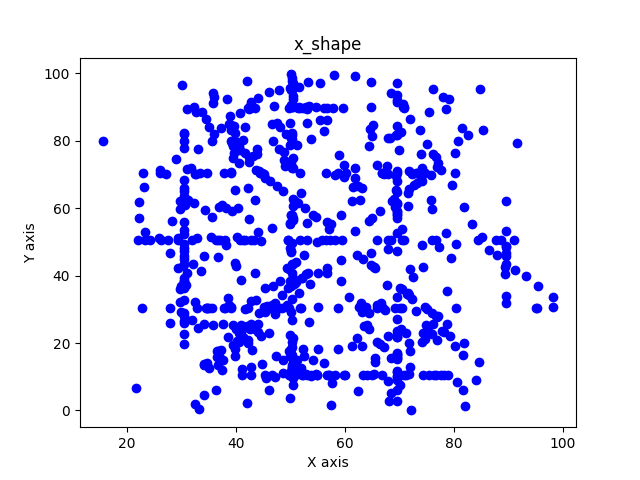
\includegraphics[width=0.20\textwidth]{images/datasaurus-4.png} &
      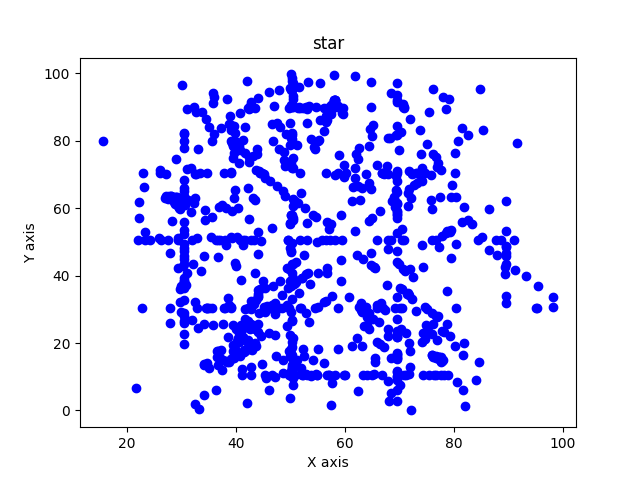
\includegraphics[width=0.20\textwidth]{images/datasaurus-5.png} &
      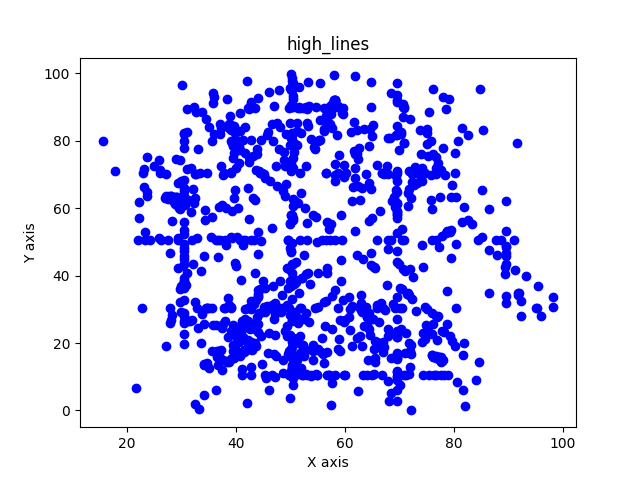
\includegraphics[width=0.20\textwidth]{images/datasaurus-6.png} &
      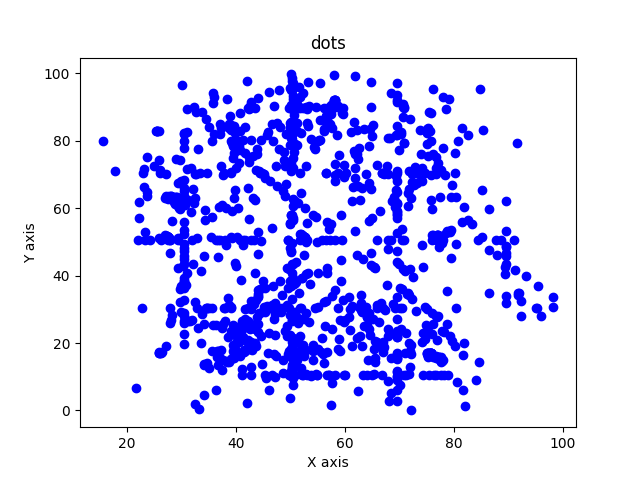
\includegraphics[width=0.20\textwidth]{images/datasaurus-7.png} \\
      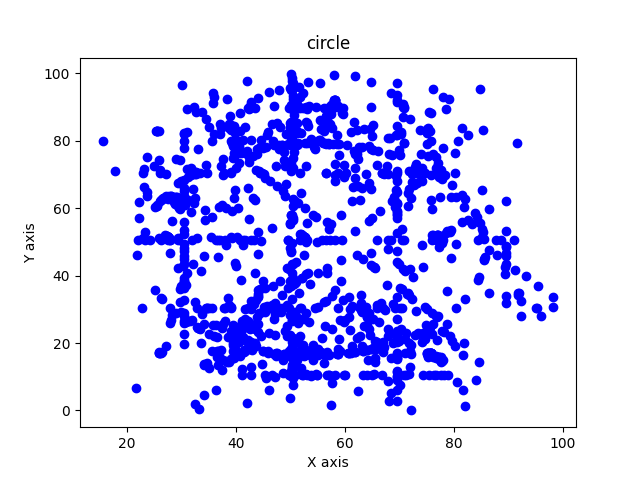
\includegraphics[width=0.20\textwidth]{images/datasaurus-8.png} &
      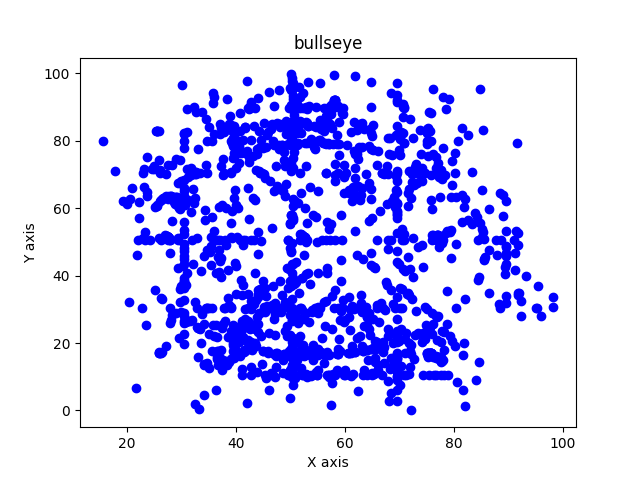
\includegraphics[width=0.20\textwidth]{images/datasaurus-9.png} &
      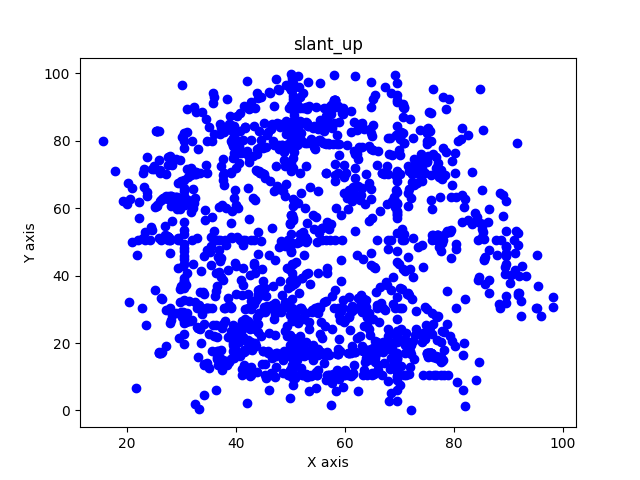
\includegraphics[width=0.20\textwidth]{images/datasaurus-10.png} &
      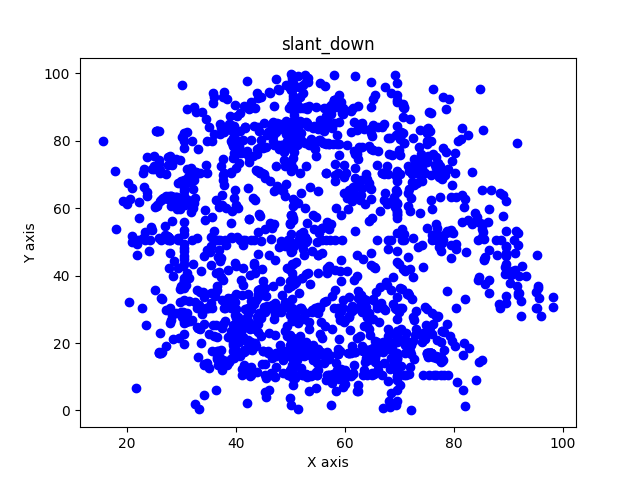
\includegraphics[width=0.20\textwidth]{images/datasaurus-11.png} \\
    \end{tabular}
  \end{center}
  \pause
  \comment{Jupter notebook: datasaurus -- bez bottleneck distance na razie.}
  \pause
  \comment{Jupter notebook: cat -- tylko pokazać.}
\end{frame}

\section{Kompleksy}
\subsection{Wstęp}
\begin{frame}{Kompleks symplicjalny}
  \emph{Kompleks symplicjalny} zbudowany jest z \emph{sympleksów},
    czyli punktów, odcinków, trójkątów, czworościanów, itd. ...
    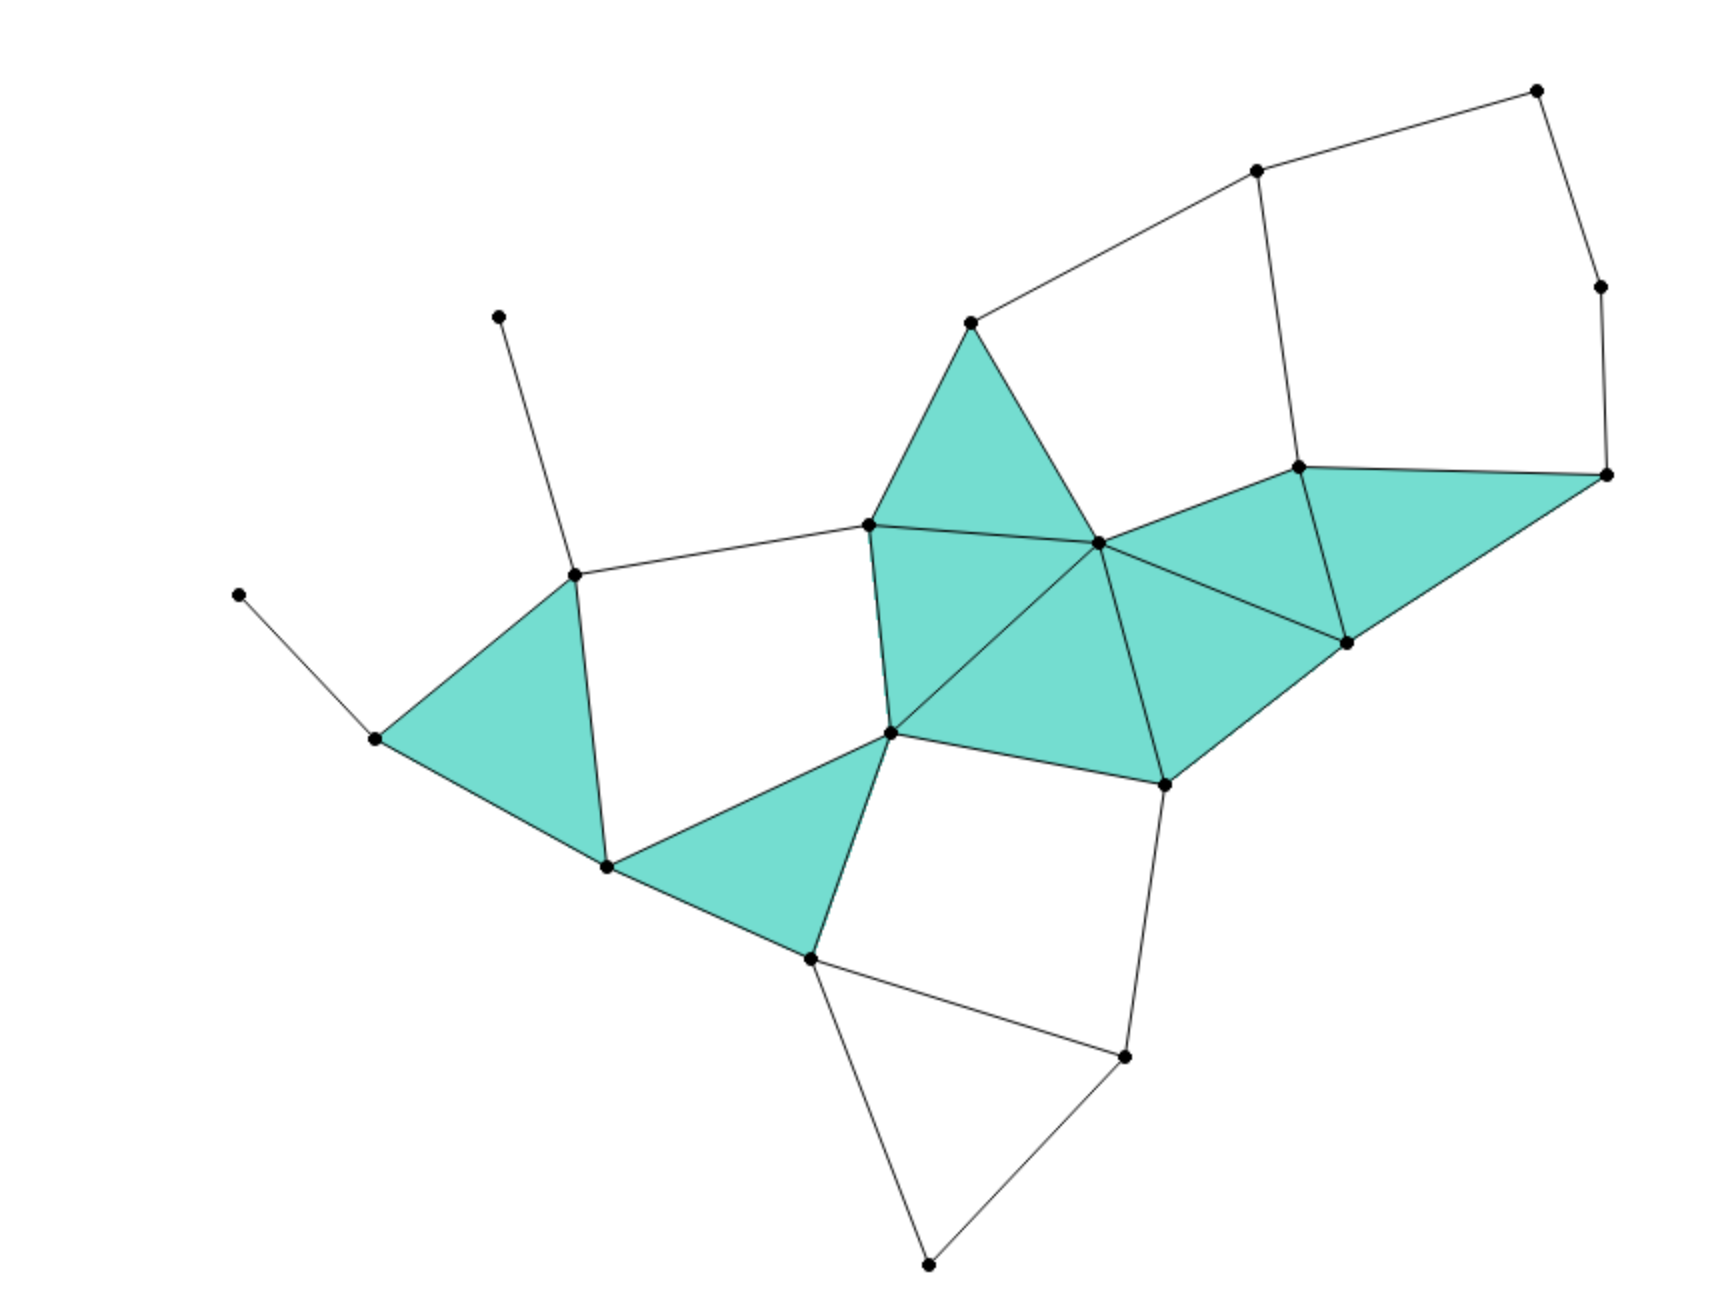
\includegraphics[width=0.9\textwidth]{images/simplicial-complex.png}
\end{frame}
\subsection{Kompleks kostkowy}
\begin{frame}{Kompleks kostkowy}
  ... natomiast \emph{kompleks kostkowy} zbudowany jest z \emph{kostek},
  czyli punktów, odcinków, kwadratów, sześcianów, itd.
    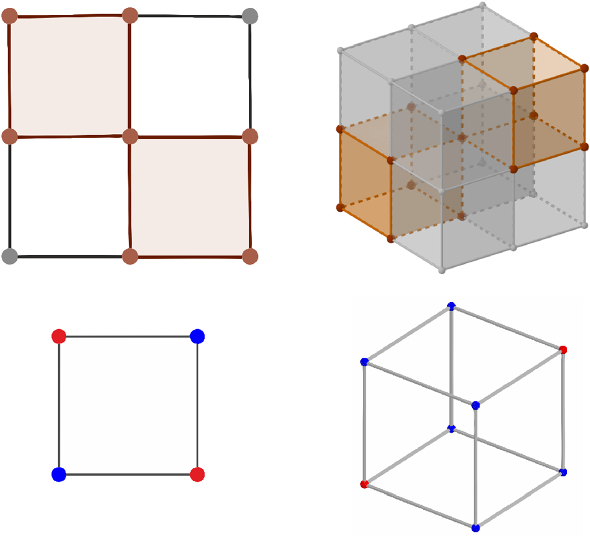
\includegraphics[width=0.60\textwidth]{images/cubical-complex.png}
  \pause

  \comment{Jak wygląda tutaj liczenie homologii?}
\end{frame}
\begin{frame}{Porównanie}
  \begin{columns}[t]
    \pause
    \begin{column}{0.48\textwidth}
      \textbf{Kompleks symplicialny}
      \pause

      Dowolny zbiór punktów na płaszczyźnie, w przestrzeni ...
          można \emph{ztriangulować}, czyli podzielić na sympleksy
      
    \end{column}
    \pause
    \begin{column}{0.48\textwidth}
      \textbf{Kompleks kostkowy}
      \pause

      Posiada naturalny sposób indeksowania kostek,
        co więcej często wystarcza pamiętać najwyżejwymiarowe kostki.
    \end{column}
    
  \end{columns}
\end{frame}

\subsection{Filtracja}
\begin{frame}{Filtracja}
  Jeśli mamy kompleks $\mathcal{K}$, to \emph{filtracją na $\mathcal{K}$}
  nazywamy ustawienie sympleksów/kostek po kolei, tak, żeby każdy
  sympleks/kostka pojawiał(a) się po wszystkich swoich ścianach.
  \pause
  \comment{Przykład filtracji -- tak naprawdę to już znacie.}
  \pause
  \comment{Mniej oczywisty przykład: jupyter notebook cubical -- bez bottleneck na razie.}
\end{frame}

\begin{frame}{Kompleks Vietorisa-Ripsa}
  Niech $A={a_0, a_1 \ldots a_n} \subseteq \mathbb{R}^n$.
  Może to być zbiór punktów w dowolnie wymiarowej przestrzeni. 
  Ustalamy promień $r \geq 0$.

  \emph{Kompleks Vietorisa-Ripsa dla $A$ i $r$} składa się z takich sympleksów
  $S\subseteq A$, że każde dwa punkty $x,y \in S$ odległe są o co najwyżej $r$.

  \pause
  \comment{Python: complex visualization: Vietoris Rips}
\end{frame}

\begin{frame}{Kompleks Čecha}
  Niech $A={a_0, a_1 \ldots a_n} \subseteq \mathbb{R}^n$.
  Może to być zbiór punktów w dowolnie wymiarowej przestrzeni. 
  Ustalamy promień $r \geq 0$.

  \emph{Kompleks Čecha dla $A$ i $r$} składa się z takich sympleksów
  $S\subseteq A$, że wszystkie kule o środkach w punktach $s\in S$ i promieniu $r$
  mają wspólny punkt.

  \pause
  \comment{Python: complex visualization: Čech}
\end{frame}

\begin{frame}{Porównanie}
  \begin{columns}[t]
    \pause
    \begin{column}{0.48\textwidth}
      \textbf{Kompleks Vietorisa-Ripsa}\pause

      Oblicza się dużo szybciej niż kompleks Čecha.
      
    \end{column}
    \pause
    \begin{column}{0.48\textwidth}
      \textbf{Kompleks Čecha}\pause

      Zachodzi \emph{Twierdzenie Čecha o nerwie}:
      kompleks Čecha jest homotopijnie równoważny z sumą kul z których powstał.
      
    \end{column}
    
  \end{columns}
  \pause
  \vspace{12pt}
  \comment{Jupyter Notebook: cat -- do końca}\\
  \pause
  \vspace{12pt}
  Pojawia się jednak bardzo ważne pytanie ...
\end{frame}

\begin{frame}{Porównanie}
  {\Huge\textcolor{red}{ILE WYMIARÓW MAJĄ TE KOMPLEKSY?}}
  \pause

  Rozwiązania są dwa: albo ignorujemy sympleksy wysokich wymiarów,
  albo w przypadku kompleksu Čecha modyfikujemy konstrukcję.
\end{frame}

\begin{frame}[Diagramy Woronoja (Voronoi Diagrams)]
    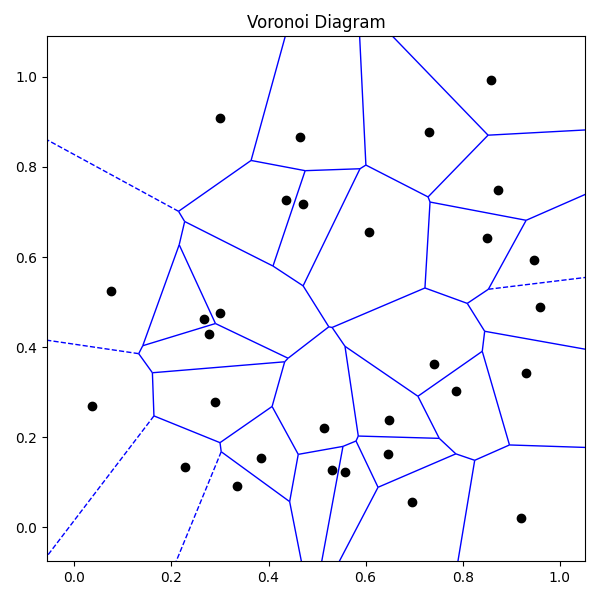
\includegraphics[width=0.70\textwidth]{images/voronoi.png}
\end{frame}

\begin{frame}[Triangulacja Delanunaya (Delaunay Triangulation)]
    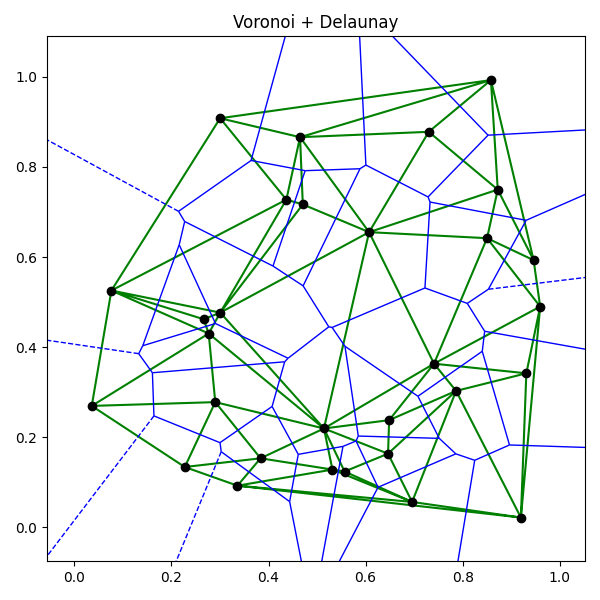
\includegraphics[width=0.70\textwidth]{images/combined.png}
\end{frame}

\begin{frame}[Triangulacja Delanunaya (Delaunay Triangulation)]
    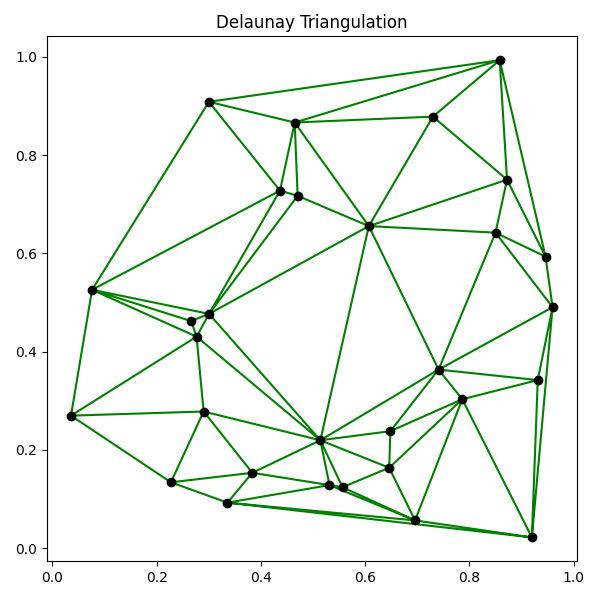
\includegraphics[width=0.70\textwidth]{images/delaunay.png}
\end{frame}


\begin{frame}[Alpha complex]
    {
    \centering
    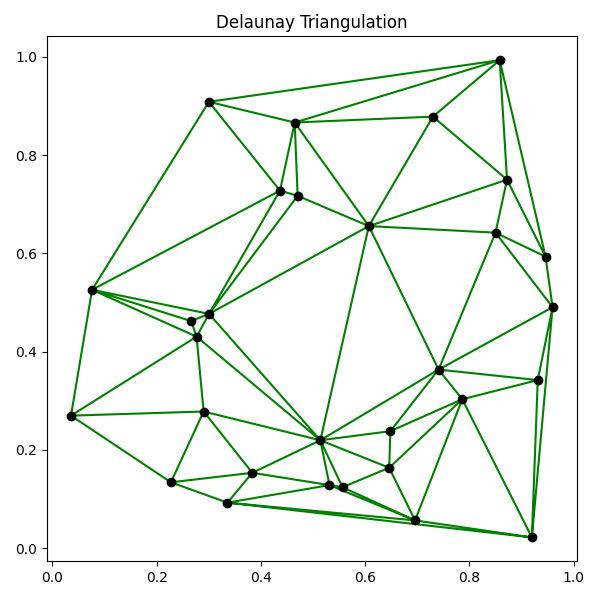
\includegraphics[width=0.50\textwidth]{images/delaunay.png}
    }
    \pause
    \vspace{12pt}
    Teraz możemy zdefiniować \emph{alpha complex} dla zbioru $A \subseteq \mathbb{R}^n$
    oraz $r \geq 0$.
    Sympleksami w nim są takie sympleksy z triangulacji Delaunaya, że
    wszystkie kule o środkach w wierzchołkach tych sympleksów i promieniu $r$
    mają wspólny punkt.
\end{frame}

\section{Stabilność diagramów persystencji}
\begin{frame}[Idea]
  Niech $\mathcal{K}$ będzie kompleksem symplicjalnym.
  \emph{Filtr na $\mathcal{K}$}
  to funkcja $\mathcal{K} \to \mathbb{R}$, która zadaje filtrację.
  Przykłady to (\comment{w prezentacji były dwa}):
  \begin{itemize}
    \pause\item Natężenie jasności piksela.
    \pause\item Wartość $r$, dla którego w kompleksie Vietorisa-Ripsa/Čecha/alpha
      dodawany jest sympleks
  \end{itemize}
  \pause
  Idea: mała zmiana filtra mało wpływa na zmianę diagramu persystencji.
\end{frame}

\begin{frame}[Odległość między filtrami]
  Jeśli $f, g$ są filtrami na $\mathcal{K}$, to chcemy sensownie zdefiniować
  odległość między nimi. Przyjmujemy
  \[
    d(f,g):=\max_{\sigma \in \mathcal{K}} \lvert f(\sigma) - g(\sigma) \rvert.
  \]
  \comment{Przykład?}
\end{frame}

\begin{frame}[Odległość między diagramami]
  Jeśli $f, g$ są filtrami na $\mathcal{K}$, to przez
  $\operatorname{Dgm}(f)$, $\operatorname{Dgm}(g)$ oznaczymy ich diagramy persystencji.
  Jak policzyć odległość między nimi?
  \pause
  \[
    d(\operatorname{Dgm}(f),\operatorname{Dgm}(g)):
      =\min_{\phi: \operatorname{Dgm}(f) \to \operatorname{Dgm}(g)}
      \max_{x \in \operatorname{Dgm}(f)} \| x - \phi(x) \|
  \]
  Nazywamy to \emph{bottleneck distance}.\\
  \pause
  \comment{Przykład? -- Jupyter Notebooks: datasaurus \& cubical ale najpierw ...}
\end{frame}

\begin{frame}[Stabilność diagramów persystencji]
  Niech $f, g$ będą filtrami na $\mathcal{K}$ oraz
  \[
    d(f,g):=\max_{\sigma \in \mathcal{K}} \lvert f(\sigma) - g(\sigma) \rvert,
  \]
  \[
    d(\operatorname{Dgm}(f),\operatorname{Dgm}(g)):
      =\min_{\phi: \operatorname{Dgm}(f) \to \operatorname{Dgm}(g)}
      \max_{x \in \operatorname{Dgm}(f)} \| x - \phi(x) \|
  \]
  \pause
  Zachodzi wówczas
  \[
    d(\operatorname{Dgm}(f),\operatorname{Dgm}(g)) \leq  d(f,g),
  \]
  z czego wynika, że
  \begin{itemize}
    \pause\item mała zmiana filtra nie zaburza nam znacznie diagramu persystencji
      -- robimy to od samego początku !!!
    \pause\item Jeśli $d(\operatorname{Dgm}(f),\operatorname{Dgm}(g))$ jest duże,
      to filtry muszą znacznie się różnić.
  \end{itemize}
  \pause \comment{Jupyter Notebooks: datasaurus \& cubical}
\end{frame}



\end{document}
